%BEGIN COPYPASTE EL INFORME DEL INFO
\documentclass[10pt, a4paper,english,spanish]{article}

\parindent=20pt
\parskip=8pt

\usepackage{graphicx}
\usepackage{ccfonts,eulervm} 
\usepackage[T1]{fontenc}
\usepackage{epigraph}
\usepackage{amsmath}
\usepackage{amsfonts}
\usepackage{amssymb}
\usepackage[activeacute, spanish]{babel}
\usepackage[utf8]{inputenc}
\usepackage{algorithm}
\usepackage{algpseudocode}
\usepackage{caption}
\usepackage{subcaption}
\usepackage{fancyhdr}

\floatname{algorithm}{Algoritmo}

\newtheorem{theorem}{Teorema}[section]
\newtheorem{lemma}[theorem]{Lema}
\newtheorem{proposition}[theorem]{Proposici\'on}
\newtheorem{corollary}[theorem]{Corolario}

\newcommand{\Var}{\textbf{var }}
\newcommand{\True}{\textbf{true }}
\newcommand{\False}{\textbf{false }}
\newcommand{\Break}{\textbf{break }}
\newcommand{\Continue}{\textbf{continue }}
\newcommand{\Param}{\textbf{param }}

\newenvironment{proof}[1][Demostraci\'on]{\begin{trivlist}
\item[\hskip \labelsep {\bfseries #1}]}{\end{trivlist}}
\newenvironment{definition}[1][Definici\'on]{\begin{trivlist}
\item[\hskip \labelsep {\bfseries #1}]}{\end{trivlist}}
\newenvironment{example}[1][Ejemplo]{\begin{trivlist}
\item[\hskip \labelsep {\bfseries #1}]}{\end{trivlist}}
\newenvironment{remark}[1][Observaci\'on]{\begin{trivlist}
\item[\hskip \labelsep {\bfseries #1}]}{\end{trivlist}}

\newcommand{\qed}{\nobreak \ifvmode \relax \else
      \ifdim\lastskip<1.5em \hskip-\lastskip
      \hskip1.5em plus0em minus0.5em \fi \nobreak
      \vrule height0.75em width0.5em depth0.25em\fi}

\parindent 0em
\algrenewcommand{\algorithmiccomment}[1]{//\textit{#1} }

\pagestyle{fancy}
\thispagestyle{fancy}
\addtolength{\headheight}{1pt}
\lhead{Proyecto CPE-B-005}
\rhead{Presentaci\'on SASE 2013}
\cfoot{\thepage}
\renewcommand{\footrulewidth}{0.4pt}
\newcommand{\hblacksquare}{\hfill \blacksquare}
%FIN COPYPASTE EL INFORME DEL INFO
\begin{document}

\section{Documento de proyecto}

\subsection{Datos administrativos}

\begin{itemize}
	\item \textbf{N\'umero de Proyecto:} CPE-B-005
	\item \textbf{Nombre:} Clon de RoadFighter
	\item \textbf{Instituci\'on:} Universidad de Buenos Aires
	\item \textbf{Materia:} Dise\~no de Sistemas con FPGA
	\item \textbf{Docente:} Patricia Borensztejn
	\item \textbf{Integrantes:} \begin{itemize}
		\item Manuel Ferreria
		\item Mat\'ias P\'erez
		\item Juan Pablo Darago
	\end{itemize} 
\end{itemize}

\subsection{Descripci\'on del proyecto}

El juego consiste en un juego inspirado en el clasico juego de Nintendo
Entertainment System (NES) RoadFighter. En esta versión, un auto debe
esquivar el tráfico en una carretera, que se va acelerando con el tiempo.
El puntaje que recibe el jugador esta basado en el tiempo en que puede
evadir los demás autos sin chocarse.

La implementación utiliza una placa de desarrollo con una FPGA Spartan 3E, 
y un pequeño periférico desarrollado por nosotros para poder conectar
joysticks estandar de Sega Genesis y poder reproducir música mediante el
uso de parlantes. 

En un apartado técnico, la implementación esta hecha completamente 
sobre lógica programable y no se han sintetizado unidades de procesamiento.
La lógica esta implementada mediante el lenguaje de descripción de hardware
Verilog. Todo esto se desarrolló en una placa Digilent Spartan 3E que 
cuenta con salida VGA que empleamos para los gráficos del juego, las entradas
y salidas adicionales de joysticks y parlantes utilizan pines de propósito
general. 

Este desarrollo fue realizado como proyecto final de la materia optativa
Diseño de Sistemas con FPGA, dictada en el primer cuatrimestre de 2012
en la Universidad de Buenos Aires, Facultad de Ciencias Exactas y
Naturales.

La música es una adaptación del videojuego clásico de Super Nintendo
Entretainment System (SNES), Chrono Trigger.

\subsection{Caracter\'isticas y funcionalidades}

\begin{itemize}
	\item Implementación en FPGA Spartan 3E mediante lógica programable, sin 
	componentes de computo.
	\item Uso de salida VGA para gráficos.
	\item Sintesis y playback de audio de un tema musical. Dos canales: base y
	melod\'ia
	\item Uso de joystick estandar de Sega Genesis.
	\item Implementación de pseudoaleatoriedad en base a entropía generada por 
	el jugador, para una experiencia más desafiante.
\end{itemize}

\subsection{Fotograf\'ias}

\begin{figure}[!h]
\centering
\begin{subfigure}{.5\textwidth}
	\centering
	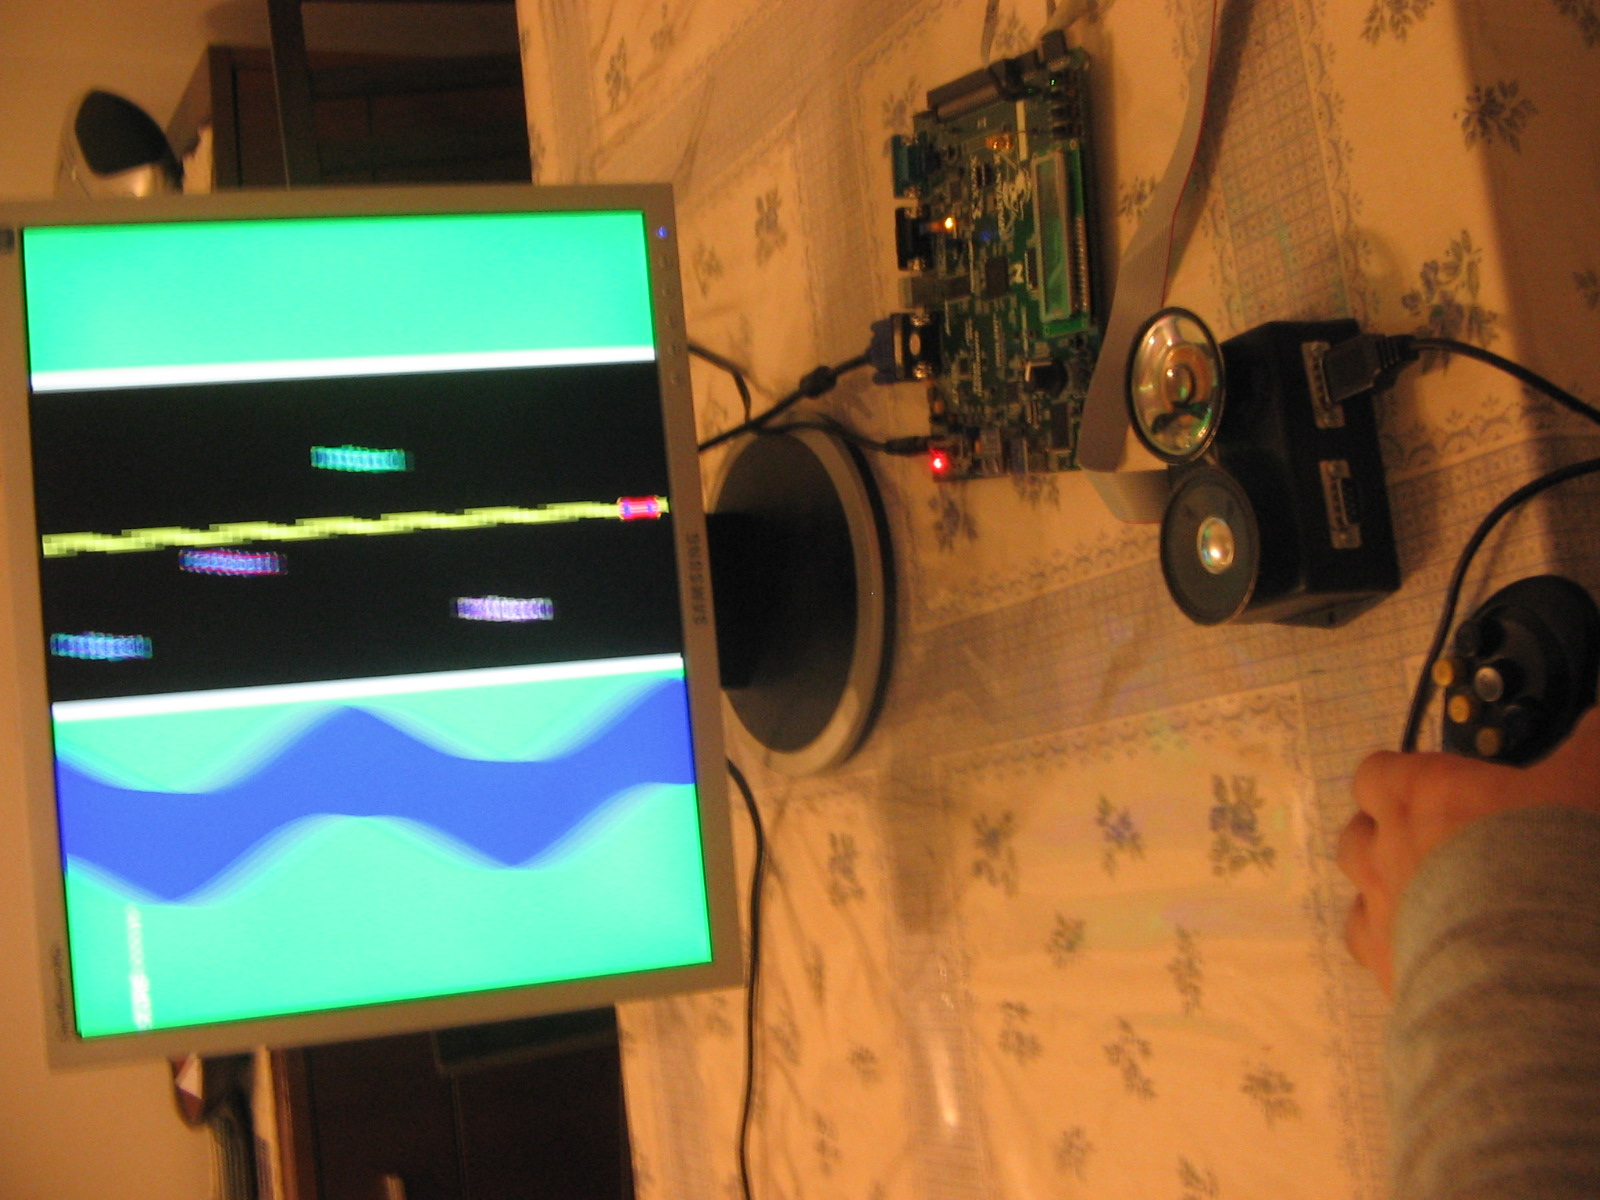
\includegraphics[width=\linewidth,angle=-90]{fotos/IMG_0203.JPG}
	\caption{Una partida en curso}
	\label{fig:current}
\end{subfigure}%
\begin{subfigure}{.5\textwidth}
	\centering
	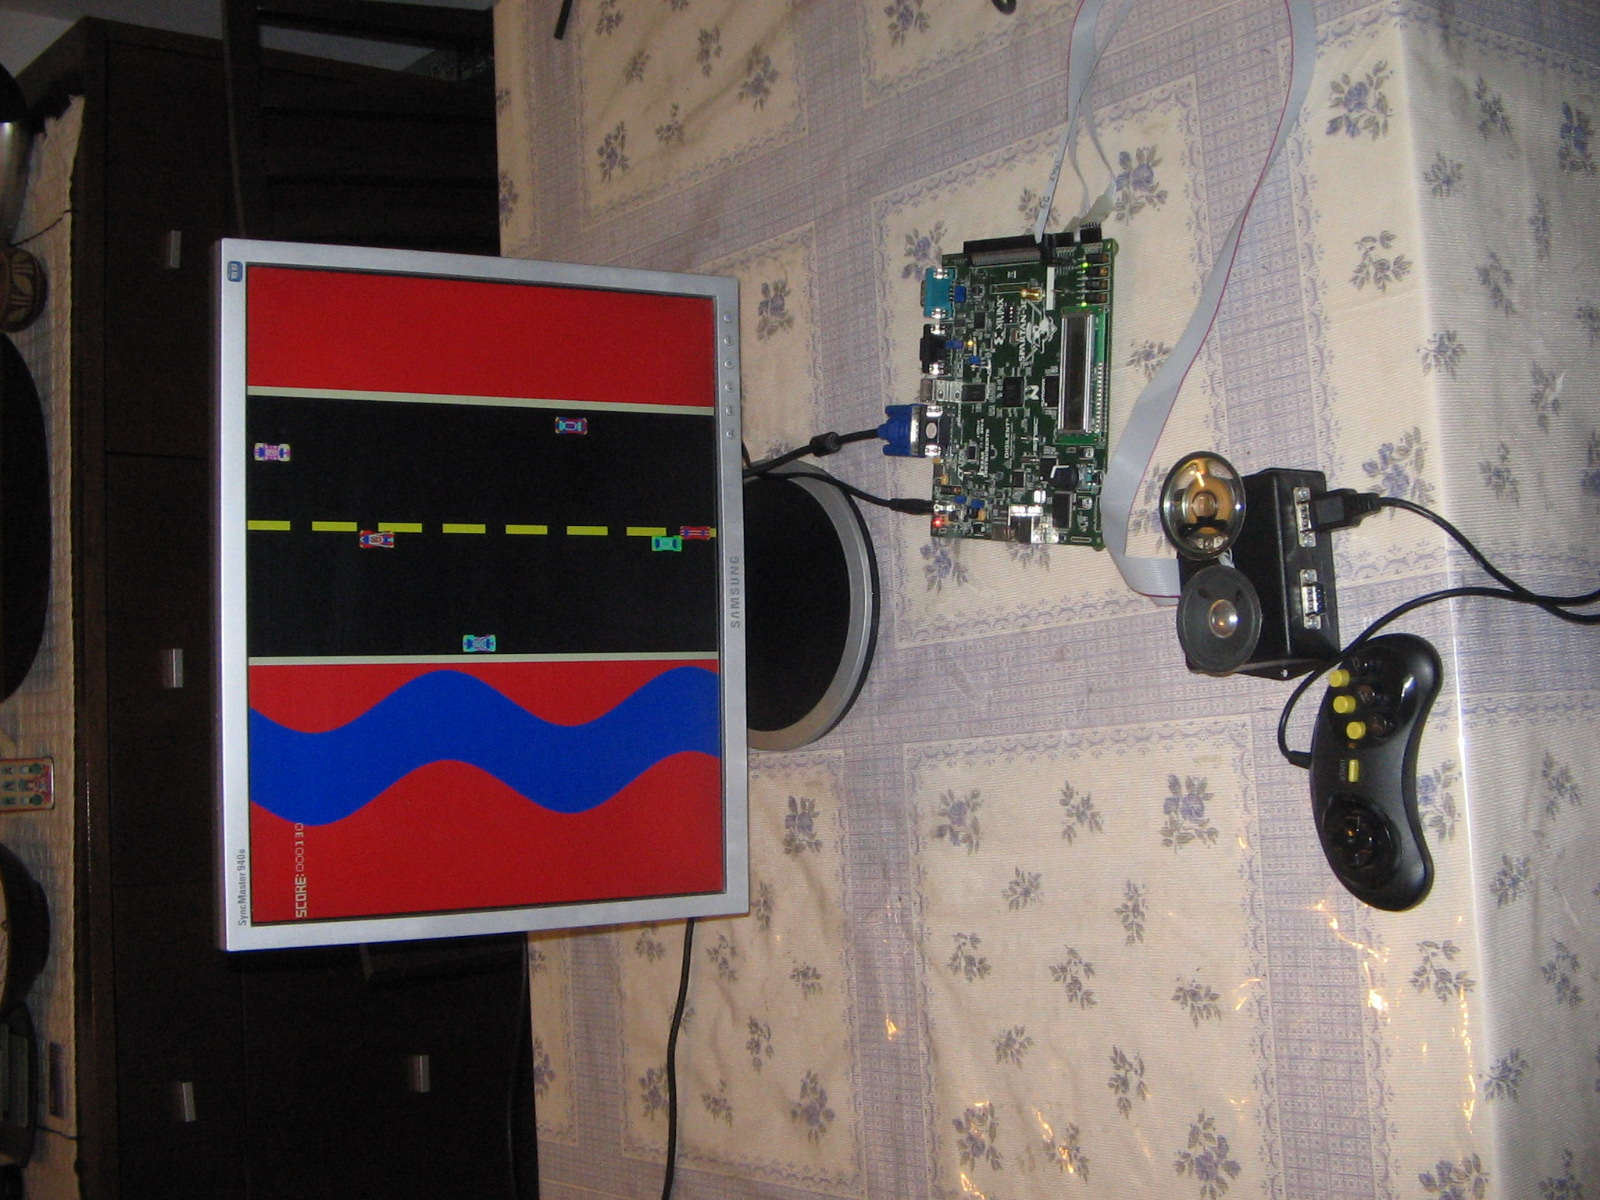
\includegraphics[width=\linewidth,angle=-90]{fotos/IMG_0208.JPG}
	\caption{Una partida perdida}
	\label{fig::lost}
\end{subfigure}
\end{figure}

\end{document}
